% Báo cáo Lab01 - Blockchain Layer-1
% Biên dịch: latexmk -xelatex REPORT.tex   (cần logo-khtn.png cùng thư mục)
\documentclass[11pt,a4paper]{article}

% ===================== THÔNG TIN NHÓM =====================
\newcommand{\TenTVa}{Võ Lê Ngọc Hiếu}   \newcommand{\MSSVa}{23127366}
\newcommand{\TenTVb}{Kiều Duy Hiếu}     \newcommand{\MSSVb}{23127365}
\newcommand{\TenTVc}{Cao Lê Gia Phú}    \newcommand{\MSSVc}{23127535}
\newcommand{\TenTVd}{Võ Thành Nhân}     \newcommand{\MSSVd}{23127533}
\newcommand{\MonHoc}{Blockchain}
% ==========================================================

\usepackage[top=2cm,bottom=2cm,left=2.3cm,right=2cm,headsep=0.5cm]{geometry}
\usepackage{fontspec}
\usepackage{polyglossia}
\setdefaultlanguage{vietnamese}
\setmainfont{Times New Roman}
\setmonofont{Courier New}[Scale=0.92]
\usepackage{amsmath}
\usepackage{setspace}
\setstretch{1.08}
\setlength{\emergencystretch}{3em}
\setlength{\parskip}{2pt}
\usepackage{xcolor,colortbl}
\usepackage{graphicx}
\usepackage{array,booktabs,tabularx,longtable}
\usepackage{float}
\usepackage{caption}
\captionsetup{font=small, labelfont=bf, skip=4pt}
\usepackage{enumitem}
\setlist{nosep, leftmargin=1.3em, topsep=2pt}
\usepackage{titlesec}
\usepackage{fancyhdr}
\usepackage{tikz}
\usetikzlibrary{arrows.meta, positioning, fit, calc}
\usepackage[hidelinks]{hyperref}
\usepackage{url}\def\UrlBreaks{\do\/\do-\do.\do_}

\definecolor{brand}{HTML}{0B5394}
\definecolor{rowgray}{HTML}{F2F5F9}
\definecolor{grpA}{HTML}{DCEBFA}
\definecolor{okgreen}{HTML}{1E7B34}
\newcolumntype{L}[1]{>{\raggedright\arraybackslash}p{#1}}
\newcolumntype{C}[1]{>{\centering\arraybackslash}p{#1}}
\newcolumntype{Y}{>{\raggedright\arraybackslash}X}

\titleformat{\section}{\large\bfseries\color{brand}}{\thesection.}{0.5em}{\MakeUppercase}
\titleformat{\subsection}{\normalsize\bfseries}{\thesubsection.}{0.5em}{}
\titlespacing*{\section}{0pt}{9pt}{4pt}
\titlespacing*{\subsection}{0pt}{6pt}{2pt}

\pagestyle{fancy}
\fancyhf{}
\fancyhead[L]{\small Lab01 -- Blockchain Layer-1}
\fancyhead[R]{\small \MonHoc}
\fancyfoot[C]{\small \thepage}
\renewcommand{\headrulewidth}{0.4pt}

\newcommand{\code}[1]{\texttt{#1}}
\newcommand{\pass}{\textbf{\color{okgreen}PASS}}

\begin{document}
\renewcommand{\refname}{Tài liệu tham khảo}

% ============================== TRANG BÌA ==============================
\begin{titlepage}
\centering
\setstretch{1.15}
\vspace*{1.2cm}
{\fontsize{17}{21}\selectfont\bfseries TRƯỜNG ĐẠI HỌC KHOA HỌC TỰ NHIÊN\par}
{\large\bfseries ĐHQG-HCM\par}
\vspace{1.4cm}

\includegraphics[width=6.2cm]{logo-khtn.png}\par
\vspace{1.4cm}
{\fontsize{22}{27}\selectfont\bfseries BÁO CÁO LAB 01\par}
\vspace{0.25cm}
{\fontsize{16}{21}\selectfont\bfseries BLOCKCHAIN LAYER-1 --\\ MÔ PHỎNG ĐỒNG THUẬN BFT NHIỀU NODE\par}
\vspace{0.3cm}
{\large Môn học: \MonHoc\par}
\vspace{2.2cm}
\renewcommand{\arraystretch}{1.25}
\begin{tabular}{@{}l@{\hspace{1.2em}}l@{\hspace{2em}}l@{}}
\textbf{Sinh viên thực hiện:} & \TenTVa & \MSSVa \\
 & \TenTVb & \MSSVb \\
 & \TenTVc & \MSSVc \\
 & \TenTVd & \MSSVd \\
\end{tabular}\par
\vfill
{\large TP. Hồ Chí Minh, tháng 11 năm 2026\par}
\end{titlepage}

% ============================== 1. THÀNH VIÊN ==============================
\section{Thông tin thành viên}

Nhóm có 4 thành viên. Mỗi người phụ trách một tầng của hệ thống và các kịch bản kiểm thử gắn với tầng đó; mọi thay đổi đi qua pull request và được thành viên khác review.

\begin{table}[H]
\centering\small
\renewcommand{\arraystretch}{1.12}
\begin{tabularx}{\linewidth}{@{}l L{3.4cm} l Y@{}}
\toprule
\textbf{MSSV} & \textbf{Họ tên} & \textbf{GitHub} & \textbf{Phụ trách} \\
\midrule
23127366 & Võ Lê Ngọc Hiếu & NgocHieu162 & A -- Nền tảng: models, encoding, chữ ký, logger, tích hợp node; kịch bản T1, T3 \\
23127365 & Kiều Duy Hiếu & DuyHieu251005 & B -- Execution (state, mempool, kiểm tra tx), fault injection, kiểm tra safety/tái lập; T4, T5, T8 \\
23127535 & Cao Lê Gia Phú & clgp-aint-cool & C -- TCP transport, HELLO, static peers, gossip, header/body; T2 \\
23127533 & Võ Thành Nhân & vtnHAN-SOLO & D -- Consensus engine, VoteSet, locking, timeout, hành vi Byzantine; T6, T7 \\
\bottomrule
\end{tabularx}
\end{table}

% ============================== 2. CẤU TRÚC ==============================
\section{Cấu trúc dự án}

Bài nộp theo đúng cấu trúc \code{Lab01\_<MSSV>/} của đề. Mã nguồn là gói Python \code{l1sim}; mỗi thư mục con ứng với một tầng của kiến trúc ở mục~4.

\begin{table}[H]
\centering\small
\renewcommand{\arraystretch}{1.08}
\begin{tabularx}{\linewidth}{@{}L{4.4cm} Y@{}}
\toprule
\textbf{Đường dẫn} & \textbf{Nội dung} \\
\midrule
\code{src/l1sim/} & \code{models} (Tx, BlockHeader, Block, Vote, Hello, Message), \code{encoding} (JSON chuẩn tắc, hash), \code{crypto} (Ed25519), \code{config}, \code{logger}, \code{node}, CLI \code{run\_node}, \code{launch\_local}, \code{client} \\
\quad\code{consensus/} & \code{engine} (máy trạng thái round), \code{vote\_set} (đếm phiếu, quorum, equivocation), \code{byzantine} (hành vi lỗi cho T3/T6/T7) \\
\quad\code{execution/} & \code{state} (key--value, nonce, state hash), \code{mempool}, \code{validation} (kiểm tra tx và block) \\
\quad\code{network/} & \code{tcp\_transport}, \code{hello}, \code{static\_peers}, \code{gossip}, \code{faults} (FaultInjector), \code{peer\_limits} \\
\quad\code{verification/} & \code{check\_safety}, \code{check\_reproducible} \\
\code{tests/} & \code{run\_tests.py} (lệnh chạy duy nhất), \code{unit/} (28 file), \code{e2e/} (T1--T8), \code{integration/} \\
\code{config/} & \code{genesis.json} (10 validator, public key) và 7 scenario \code{t1\_normal} … \code{t7\_byzantine} \\
\code{logs/} & \code{events/<scenario>/V*.jsonl}, \code{results/<scenario>/V*.json}, \code{verdict.json}, stdout/stderr từng node \\
\code{dashboard/} & giao diện web để demo (\code{server.py}, \code{index.html}); chỉ dùng khi trình bày, không nằm trong file zip nộp \\
\code{README.md}, \code{REPORT.pdf} & hướng dẫn chạy, đọc log, tái lập; báo cáo này \\
\bottomrule
\end{tabularx}
\end{table}

% ============================== 3. GIỚI THIỆU ==============================
\section{Giới thiệu}

\subsection{Mục đích hệ thống}
Hệ thống mô phỏng một blockchain Layer-1, trong đó mỗi validator là một \textbf{process riêng} giao tiếp qua \textbf{TCP thật}. Các validator cùng duy trì một state dạng key--value, nhận giao dịch có chữ ký, gom thành block và đồng thuận theo ba bước Propose → Prevote → Precommit. Mục tiêu là chứng minh bằng thực nghiệm hai tính chất của đề:
\begin{itemize}
\item \textbf{Safety} luôn đúng: hai node trung thực không bao giờ finalize hai block khác nhau ở cùng height, kể cả khi mạng mất, trễ, trùng, đảo thứ tự message và có tối đa $f$ validator Byzantine.
\item \textbf{Liveness} sau GST: khi mạng ổn định, chain tiếp tục tiến.
\end{itemize}
Cấu hình chuẩn có $n = 10$ validator, nên $f = \lfloor (n-1)/3 \rfloor = 3$ và quorum $= n - f = 2f+1 = 7$.

\subsection{Các lựa chọn thiết kế chính}
\begin{itemize}
\item \textbf{Python 3.10 + asyncio}: mỗi node chạy một event loop; chỉ phụ thuộc thư viện \code{cryptography} cho Ed25519.
\item \textbf{Mã hóa chuẩn tắc}: mọi giá trị được ký hoặc hash đều qua cùng một hàm encode (JSON, khóa sắp xếp, không khoảng trắng, UTF-8, cấm số thực). Bộ giải mã từ chối message không chuẩn tắc, nên mỗi giá trị chỉ có đúng một dạng bytes.
\item \textbf{Tách domain}: chữ ký và hash có tiền tố \code{<DOMAIN>:lab01} (TX, HEADER, VOTE, HELLO, BLOCK, STATE…), nên một chữ ký hợp lệ không thể dùng lại ở ngữ cảnh khác hay chain khác.
\item \textbf{Đồng thuận kiểu Tendermint} có locking, timeout tăng dần theo round và round-skip. Engine là máy trạng thái thuần: không chạm mạng, đồng hồ hay \code{asyncio}, mọi tác dụng phụ đi qua callback, nên unit test được từng luật.
\item \textbf{Mạng full mesh tĩnh} (static peers) + gossip flood có dedup; block truyền theo kiểu \textbf{header trước, body sau}.
\item \textbf{Tất định}: khóa sinh từ seed, lỗi mạng là hàm hash của \code{(seed, src, dst, message\_id)}, hành vi Byzantine suy ra từ message trung thực, results chỉ chứa dữ liệu đã sắp xếp. Nhờ đó cùng seed cho results giống từng byte (T8).
\end{itemize}

% ============================== 4. THIẾT KẾ ==============================
\section{Thiết kế hệ thống}

\subsection{Sơ đồ kiến trúc}

\begin{figure}[H]
\centering
\resizebox{\linewidth}{!}{%
\begin{tikzpicture}[
  box/.style={draw=brand, fill=grpA, rounded corners=2pt, minimum height=0.8cm, minimum width=2.6cm, align=center, font=\footnotesize, inner sep=2pt},
  lay/.style={draw=gray!60, dashed, rounded corners=3pt, inner sep=5pt},
  lbl/.style={font=\scriptsize\bfseries\color{brand}, anchor=south west, inner sep=1pt},
  arr/.style={-{Stealth[length=5pt]}, thick, gray!60!black},
  al/.style={font=\scriptsize, midway, fill=white, inner sep=1pt}]
% network row
\node[box] (gos) at (1.5,0) {Gossip\\(flood + dedup)};
\node[box] (fi)  at (4.5,0) {FaultInjector\\(drop / dup / trễ)};
\node[box] (tcp) at (7.5,0) {TcpTransport\\(frame 4 byte)};
\node[box] (hel) at (10.5,0) {HELLO\\+ StaticPeers};
% node row
\node[box, minimum width=11.6cm] (node) at (6,-1.75) {Node: định tuyến message, kiểm header, header/body, hẹn giờ timeout, ghi results};
% consensus row
\node[box] (vs)  at (1.5,-3.5) {VoteSet\\(đếm phiếu, quorum)};
\node[box] (eng) at (6,-3.5) {ConsensusEngine\\(round, step, lock)};
\node[box] (byz) at (10.5,-3.5) {Byzantine\\(chỉ khi cấu hình)};
% execution row
\node[box] (mem) at (1.5,-5.25) {Mempool};
\node[box] (val) at (6,-5.25) {Validation\\(tx, block)};
\node[box] (st)  at (10.5,-5.25) {State\\(key--value + nonce)};
% shared column
\node[box, minimum width=2.4cm] (log) at (14.3,-1.75) {EventLogger\\(JSONL)};
\node[box, minimum width=2.4cm] (cry) at (14.3,-3.5) {crypto\\(Ed25519)};
\node[box, minimum width=2.4cm] (enc) at (14.3,-5.25) {encoding\\(JSON chuẩn tắc)};
% containers + labels
\node[lay, fit=(gos)(hel)] (Ln) {}; \node[lbl] at (Ln.north west) {network/};
\node[lay, fit=(vs)(byz)] (Lc) {}; \node[lbl] at (Lc.north west) {consensus/};
\node[lay, fit=(mem)(st)] (Le) {}; \node[lbl] at (Le.north west) {execution/};
\node[lay, fit=(log)(enc)] (Ls) {}; \node[lbl] at (Ls.north west) {dùng chung};
% arrows
\draw[arr, <->] (gos) -- (gos|-node.north);
\draw[arr] (gos) -- (fi);
\draw[arr] (fi) -- (tcp);
\draw[arr, <->] (tcp) -- (hel);
\draw[arr] (node) -- node[al]{proposal, vote, timeout} (eng);
\draw[arr] (vs) -- (eng);
\draw[arr] (eng) -- node[al]{gửi đi} (byz);
\draw[arr] (byz) -- node[al]{broadcast} (byz|-node.south);
\draw[arr] (eng) -- node[al]{rule 3} (val);
\draw[arr] (mem) -- (val);
\draw[arr] (val) -- (st);
\end{tikzpicture}
}
\caption{Các module trong một validator. Mỗi process chạy đúng một bộ như trên; 10 process nối full mesh qua TCP.}
\label{fig:arch}
\end{figure}

\subsection{Vai trò của các module}
\begin{itemize}
\item \textbf{TcpTransport} chỉ chuyển bytes: mỗi frame là 4 byte độ dài big-endian + nội dung, tối đa 1\,MB. Mỗi peer có một coroutine đọc; ghi một frame là một lệnh \code{write} nên frame không xen nhau. Peer đọc quá chậm (buffer gửi > 4\,MB) bị bỏ message thay vì làm node chậm theo.
\item \textbf{HELLO} xác thực peer ngay sau khi kết nối: mỗi bên gửi \code{Hello} (chain\_id, node\_id, địa chỉ, height đã finalize) ký bằng domain \code{HELLO}. Bên nhận kiểm theo thứ tự \code{malformed} → \code{wrong\_chain} → \code{unknown\_peer} → \code{self\_connect} → \code{bad\_signature}.
\item \textbf{StaticPeers} dựng full mesh từ \code{network.peers}: node đứng sau trong thứ tự sắp xếp chủ động nối tới node đứng trước, nên mỗi cặp chỉ có một kết nối; mất kết nối thì quay số lại sau 0,1\,s.
\item \textbf{Gossip} phân hai loại message: FLOOD (TX, HEADER, VOTE) gửi cho mọi peer và chuyển tiếp nếu tầng trên chấp nhận; DIRECT (BODY\_REQUEST, BODY) gửi 1--1.
\item \textbf{FaultInjector} nằm giữa Gossip và transport, quyết định drop / gửi / nhân đôi và độ trễ cho từng message trên từng link.
\item \textbf{Node} nối mọi thứ: kiểm tra sơ bộ (height, proposer, chữ ký header), quản lý header/body, hẹn giờ timeout cho engine, đưa tx vào mempool và ghi results khi đạt \code{max\_height}.
\item \textbf{ConsensusEngine} chạy luật vote; \textbf{VoteSet} là nơi duy nhất đếm phiếu; \textbf{Byzantine} (nếu có trong scenario) biến đổi message gửi đi của một node, còn engine bên trong vẫn chạy luật trung thực.
\item \textbf{Execution}: \code{validate\_tx} (chữ ký → quyền sở hữu key → nonce), \code{validate\_block} (proposer, parent, chữ ký header, tx\_root, chạy thử tx, state hash), \code{apply\_block}.
\end{itemize}

\subsection{Luồng message trong một height}

\begin{figure}[H]
\centering
\begin{tikzpicture}[
  font=\footnotesize, >={Stealth[length=5pt]},
  lane/.style={draw=gray!50, thick},
  msg/.style={->, thick, brand},
  ml/.style={above, inner sep=1.5pt, font=\scriptsize},
  st/.style={fill=grpA, draw=brand, rounded corners=1pt, inner sep=2.5pt, font=\scriptsize}]
\def\C{0} \def\P{3.4} \def\V{8.4} \def\O{14.6}
\foreach \x/\n in {\C/Client, \P/{Proposer $P$}, \V/{Validator $V_i$}, \O/{Các validator khác}} {
  \node[font=\footnotesize\bfseries] at (\x,0.3) {\n};
  \draw[lane] (\x,0.05) -- (\x,-8.5);
}
\draw[msg] (\C,-0.45) -- node[ml]{TX (ký domain TX)} (\P,-0.45);
\draw[msg, dashed] (\P,-0.95) -- node[ml]{gossip TX → mempool mọi node} (\V,-0.95);
\node[st] at (\P,-1.55) {new\_round: $P=\mathrm{sorted}(V)[(h+r)\bmod n]$, tạo block};
\draw[msg] (\P,-2.2) -- node[ml]{HEADER (ký domain HEADER)} (\V,-2.2);
\draw[msg] (\V,-2.75) -- node[ml]{BODY\_REQUEST(hash)} (\P,-2.75);
\draw[msg] (\P,-3.3) -- node[ml]{BODY (khớp header, tx\_root)} (\V,-3.3);
\node[st] at (\V,-3.9) {validate\_block → PREVOTE(hash hoặc nil)};
\draw[msg] (\V,-4.5) -- node[ml]{PREVOTE} (\O,-4.5);
\draw[msg] (\O,-5.0) -- node[ml]{PREVOTE của $n-1$ node} (\V,-5.0);
\node[st] at (\V,-5.6) {$\ge 2f+1$ prevote cho $B$ (polka) → lock $B$, PRECOMMIT $B$};
\draw[msg] (\V,-6.2) -- node[ml]{PRECOMMIT} (\O,-6.2);
\draw[msg] (\O,-6.7) -- node[ml]{PRECOMMIT của $n-1$ node} (\V,-6.7);
\node[st] at (\V,-7.3) {$\ge 2f+1$ precommit cho $B$ → FINALIZE, apply\_block, sang height $h+1$};
\node[st, fill=red!8, draw=red!60!black, anchor=west] at (\C,-8.1) {Hết timeout ở một bước: prevote/precommit nil, hoặc sang round $r+1$ với proposer kế tiếp};
\end{tikzpicture}
\caption{Một height ở trường hợp bình thường. Mọi vote đều được gossip flood; mũi tên chỉ vẽ luồng chính.}
\label{fig:flow}
\end{figure}

\subsection{Hoạt động chi tiết và các tương tác chính}
\textbf{Mô hình dữ liệu.} Tx gồm \code{(sender, key, value, nonce, signature)}; \code{key} phải có dạng \code{<sender>/...} (người gửi chỉ ghi vào vùng của mình). Header gồm \code{height, round, parent\_hash, tx\_root, state\_hash, proposer, signature}; block hash là SHA-256 của header bỏ chữ ký, domain \code{BLOCK}. \code{tx\_root} là hash (domain \code{TXS}) của danh sách tx đã mã hóa chuẩn tắc. \code{state\_hash} là hash (domain \code{STATE}) của toàn bộ map dữ liệu và map nonce. Vote gồm \code{(phase, height, round, block\_hash | null, voter, signature)}. Mỗi message trên dây là \code{Message(kind, origin, height, payload)}.

\textbf{Chọn proposer.} Mọi node tính $P(h,r) = \mathrm{sorted}(V)[(h + r) \bmod n]$ cục bộ, không cần trao đổi. Round tăng thì proposer xoay vòng, nên proposer im lặng chỉ làm mất một round.

\textbf{Một round.} Khi vào round, proposer lấy tối đa \code{max\_txs\_per\_block} tx hợp lệ từ mempool (đúng nonce kế tiếp), chạy thử trên bản sao state để tính \code{state\_hash}, ký header và broadcast. Node khác nhận HEADER, kiểm chữ ký và proposer rồi xin BODY từ chính peer đã gửi header; nếu sau 300\,ms chưa có body thì hỏi mọi validator khác. Khi có block, engine quyết định PREVOTE theo luật lock (mục~5.3); gặp polka thì PRECOMMIT; gặp $2f+1$ PRECOMMIT cho một block đã có thì finalize. Mỗi bước có timeout $T_{\text{step}}(r) = T_{\text{base}} + r \cdot \delta$ (1000\,ms + $r \cdot$ 300\,ms).

\textbf{Chain và view.} Mỗi node giữ chain đã finalize, state hiện tại và \code{CommitCertificate} ($2f+1$ precommit). Khi đạt \code{max\_height}, node ghi \code{results/V*.json} (height, block hash, proposer, round, commit\_round, tx id, state hash). \code{check\_safety} đọc results của mọi node và kiểm: không có hai block khác nhau ở cùng height, cùng state hash ở height chung, đủ quorum node đạt \code{max\_height}.

% ============================== 5. CÀI ĐẶT ==============================
\section{Ghi chú cài đặt}

\subsection{Các lớp bảo vệ (guard)}
Mỗi message phải qua lần lượt các guard dưới đây; bị loại ở bước nào thì node ghi event kèm \code{reason} tương ứng và \textbf{không chuyển tiếp} message đó.

\begin{table}[H]
\centering\small
\renewcommand{\arraystretch}{1.08}
\begin{tabularx}{\linewidth}{@{}L{2.6cm} Y L{4.0cm}@{}}
\toprule
\textbf{Guard} & \textbf{Cách hiện thực} & \textbf{Event / reason} \\
\midrule
Kích thước, định dạng & Frame > 1\,MB bị bỏ; \code{decode} kiểm đúng tập trường, kiểu, và encode lại phải trùng bytes đã nhận & \code{gossip\_malformed} \\
Xác thực peer & HELLO ký domain HELLO, peer phải thuộc genesis, không tự nối chính mình, đúng chain\_id & \code{handshake\_failed} \\
Nguồn gửi & Peer và \code{origin} phải là validator trong genesis; client chỉ được gửi TX & (bỏ qua) \\
Trùng lặp & Gossip dedup theo \code{message\_id} (hash domain MSG) trước lệnh \code{await} đầu tiên; VoteSet dedup theo (voter, height, round, phase, giá trị) & \code{gossip\_duplicate}, \code{duplicate\_ignored} \\
Height cũ / ngoài phạm vi & Message có height < height hiện tại hoặc > \code{max\_height} bị bỏ & \code{ignored\_old\_height} \\
Chữ ký vote & Kiểm Ed25519 với domain VOTE; nếu sai thì thử các domain khác để phân biệt hai lỗi & \code{vote\_rejected}: \code{bad\_signature}, \code{wrong\_domain} \\
Header & Chữ ký domain HEADER, proposer phải đúng $P(h,r)$ & \code{header\_rejected} \\
Body & Header của body phải trùng header đã nhận; \code{tx\_root} khớp danh sách tx & \code{body\_rejected} \\
Block (rule 3) & Đúng proposer, đúng parent, chữ ký, tx\_root, từng tx hợp lệ khi chạy tuần tự, state hash sau thực thi khớp header & \code{invalid\_block} \\
Giao dịch & Chữ ký domain TX → quyền sở hữu key → nonce; mempool nhận nonce tương lai nhưng block chỉ nhận đúng nonce kế tiếp; trùng (sender, nonce) bị từ chối & \code{bad\_signature}, \code{not\_owner}, \code{bad\_nonce} \\
Tự ký hai lần & Engine không bao giờ ký hai vote khác nhau cho cùng (height, round, phase) & \code{refuse\_double\_sign} \\
Equivocation & VoteSet lưu bằng chứng khi một voter ký hai giá trị cho cùng slot & \code{equivocation\_detected} \\
\bottomrule
\end{tabularx}
\end{table}

\textbf{Rate limit.} Đề yêu cầu giới hạn tốc độ và chặn peer. Nhóm có module \code{PeerLimits} (giới hạn 1000 message/giây mỗi peer cả chiều vào và ra, chặn peer vượt ngưỡng trong 10\,s, có unit test), cùng ngưỡng buffer 4\,MB ở transport. Tuy nhiên ở bản nộp, \code{PeerLimits} \textbf{chưa được gắn vào đường nhận của node}; đây là hạn chế được nêu lại ở mục~6.3.

\subsection{Chiến lược gossip và header trước body}
Mỗi node nối trực tiếp với mọi validator khác. Khi tạo message FLOOD, node đánh dấu \code{message\_id} là đã thấy rồi gửi cho mọi peer. Node nhận chạy handler; chỉ khi handler chấp nhận (\code{True}) thì mới chuyển tiếp \textbf{đúng bytes đã nhận} cho mọi peer trừ nơi gửi. Vì đánh dấu đã thấy trước khi xử lý, một message bị từ chối sẽ không được xét lại, nên handler chỉ trả \code{False} cho lỗi vĩnh viễn (chữ ký sai, height cũ, nonce cũ). Mỗi message được xử lý đúng một lần dù tới nhiều bản: ở T1, 10 node ghi khoảng 6000 \code{gossip\_duplicate} và không bản nào được xử lý lại.

Block không được flood nguyên khối: node gửi \code{BLOCK} nội bộ, tầng gửi tách thành HEADER (flood). Node nhận header hợp lệ mà chưa có body thì gửi \code{BODY\_REQUEST} tới peer vừa gửi header, sau 300\,ms hỏi thêm mọi validator khác. Node đã có header nhưng chưa có body sẽ ghi nhớ người hỏi và trả body khi nhận được. Body của 20 height gần nhất được giữ lại để trả lời node chậm.

\textbf{Mô phỏng lỗi mạng.} \code{FaultInjector} băm \code{seed|src|dst|message\_id} bằng SHA-256 rồi lấy các đoạn của digest làm số ngẫu nhiên: $u < $ \code{drop\_rate} thì drop (chỉ khi height < \code{gst\_height}); $u$ nằm trong khoảng tiếp theo có độ rộng \code{duplicate\_rate} thì gửi hai bản. Độ trễ có hai cực: ngắn (1 đến 10\% timeout, đủ để đảo thứ tự) hoặc, trước GST, dài (hơn hai lần timeout lớn nhất). Thiết kế hai cực tránh vùng trễ xấp xỉ timeout, nơi kết quả phụ thuộc vào thời điểm chạy và phá T8. Quyết định chỉ phụ thuộc nội dung message, không phụ thuộc thứ tự gọi, nên mọi lần chạy cùng seed có cùng số phận cho cùng message.

\subsection{Các bước đồng thuận và luật vote}
Engine có một vòng \code{\_progress} duy nhất, chạy sau mỗi input (proposal, vote, timeout) và áp lần lượt mọi luật có điều kiện đúng cho tới khi không còn gì thay đổi. Bảy luật của đề được hiện thực như sau:
\begin{enumerate}
\item \textbf{Mỗi (height, round, phase) chỉ một vote}: hàm ký vote của engine từ chối ký giá trị thứ hai (\code{refuse\_double\_sign}).
\item \textbf{Chỉ finalize với $2f+1$ precommit cho cùng block}: \code{\_try\_finalize} xét mọi round của height hiện tại, kể cả round cũ, để node đã sang round sau vẫn finalize khi precommit muộn tới. Nếu có quorum cho block chưa nhận được, node chờ (\code{commit\_waiting\_for\_block}).
\item \textbf{Chỉ prevote block hợp lệ}: \code{validate\_block}; block sai thì prevote nil.
\item \textbf{Lock}: khi precommit $B$ vì thấy polka cho $B$ ở round $r$, node lưu \code{locked\_block = B}, \code{locked\_round = r} (event \code{lock}).
\item \textbf{Đã lock thì prevote block đã lock}, trừ khi thấy polka cho block khác ở round mới hơn \code{locked\_round}. Proposer đang lock thì đề xuất lại đúng block đó (\code{repropose}, cùng header, cùng hash).
\item \textbf{Timeout}: hết PROPOSE thì prevote nil; hết PREVOTE thì precommit nil; hết PRECOMMIT thì sang round $r+1$. Ngoài ra có round-skip: thấy $f+1$ voter khác nhau ở round cao hơn (chắc chắn có node trung thực) thì nhảy tới round đó.
\item \textbf{Không đếm vote trùng}: VoteSet đếm mỗi voter tối đa một lần cho mỗi giá trị trong một slot; quorum là $n - f$ voter khác nhau.
\end{enumerate}

\textbf{Vì sao an toàn.} Hai quorum kích thước $2f+1$ trong $n = 3f+1$ validator giao nhau ít nhất $f+1$ voter, trong đó có ít nhất một node trung thực; node đó không ký hai giá trị cho cùng slot, nên hai block không thể cùng đạt quorum ở một round. Giữa các round, $f+1$ node trung thực đã lock block được finalize sẽ chỉ prevote block đó, nên không block nào khác đạt polka ở round sau.

\textbf{Polka evidence.} Mỗi khi vào round mới, node đang theo một polka cũ gửi lại $2f+1$ prevote có chữ ký của polka đó. Node bỏ lỡ polka kiểm chữ ký từng phiếu, thấy polka và prevote cùng block. Cơ chế này chỉ gửi lại vote thật nên không đổi luật nào (xem lỗi D6).

\textbf{Byzantine.} Node Byzantine chạy engine trung thực, chỉ có message gửi đi bị biến đổi: \code{silent} (không gửi), \code{equivocate} (thêm một block/vote mâu thuẫn, ký hợp lệ), \code{bad\_signature} (đổi một ký tự hex của chữ ký), \code{wrong\_domain} (ký lại bằng domain khác). Mọi biến đổi suy ra từ message gốc, không dùng số ngẫu nhiên, nên vẫn tái lập được.

\subsection{Các lỗi khó và cách khắc phục}
Các lỗi dưới đây chỉ lộ ra khi chạy nhiều process với lỗi mạng hoặc Byzantine; chi tiết đầy đủ nằm trong \code{docs/BUGS.md}.
\begin{enumerate}[leftmargin=1.5em]
\item \textbf{Mất safety khi chưa có locking.} Dựng lại phản ví dụ: V0 finalize $B$ ở round 0, các node khác mất precommit round 0 rồi finalize $C$ ở round 1. Nguyên nhân là bản đầu chưa có luật 4--5. Thêm locking; test \code{test\_locking\_keeps\_safety\_when\_round\_0\_precommits\_are\_lost}.
\item \textbf{Locking theo đúng flowchart làm chain đứng.} Node đã lock prevote nil khi proposal là block khác, còn proposer luôn tạo block mới, nên nhóm đã lock và nhóm chưa lock không bên nào đủ quorum. Sửa: node lock prevote \emph{block đã lock}; proposer đang lock đề xuất lại block đó; node chưa lock nhưng biết polka cũ thì prevote block của polka. Safety không đổi vì node lock vẫn không prevote block khác.
\item \textbf{Polka chỉ tới một phần mạng thì kẹt vĩnh viễn.} Round 0 chỉ V0--V3 thấy polka và lock $B$; V4--V9 không bao giờ biết $B$ từng có polka vì gossip không gửi lại prevote cũ. Sửa bằng polka evidence (mục 5.3); có test đối chứng cho thấy không có cơ chế này thì kẹt.
\item \textbf{T7 thỉnh thoảng kẹt vì không đếm vote thật của node equivocate.} VoteSet ban đầu chỉ giữ vote tới trước của mỗi voter. Một node nhận precommit giả của V7--V9 trước, nên precommit thật cho block được commit bị coi là equivocation và không đếm; node đó thiếu quorum mãi mãi. Sửa: đếm mỗi vote cho đúng giá trị của nó, mỗi voter tối đa một lần mỗi giá trị, vẫn lưu bằng chứng; vote xung đột mới được chuyển tiếp đúng một lần. Vẫn an toàn vì hai block cùng đạt quorum đòi hỏi ít nhất một node trung thực equivocate.
\item \textbf{Block xung đột bị vứt nên không finalize được.} Proposer Byzantine gửi hai block cho cùng (height, round); node nhận block thứ hai sau bỏ hẳn nó. Nếu mạng commit đúng block thứ hai, node có đủ precommit mà không có block (\code{commit\_waiting\_for\_block} mãi). Sửa: block xung đột không chiếm slot proposal (không được prevote) nhưng vẫn được lưu theo hash.
\item \textbf{T7 chạy hai lần cho kết quả khác nhau.} Thứ tự hai proposal xung đột tới mỗi node phụ thuộc gossip, và số cặp equivocation mỗi node bắt được phụ thuộc thời điểm. Sửa: bản mâu thuẫn được gửi trễ gấp đôi timeout dài nhất; results chỉ ghi danh sách \code{equivocators} đã sắp xếp, chi tiết từng cặp để trong event log.
\item \textbf{Engine crash ở event đầu tiên khi ghép với logger}: cả engine lẫn logger cùng ghi trường \code{node}. Sửa: logger sở hữu node id.
\end{enumerate}

% ============================== 6. KIỂM THỬ ==============================
\section{Kiểm thử và kết quả}

\subsection{Cách chạy}
Một lệnh duy nhất chạy toàn bộ: \code{python tests/run\_tests.py}; chọn kịch bản bằng \code{-{}-scenario T1 … T8}, chỉ unit bằng \code{-{}-unit}, chỉ E2E bằng \code{-{}-e2e}. Mỗi test E2E khởi động 10 process \code{run\_node} trên TCP loopback, chờ chạy xong rồi kiểm nội dung results, state, số giao dịch và event log, không chỉ dựa vào exit code. Unit test (28 file) kiểm riêng chữ ký và domain, encoding chuẩn tắc, nonce, ownership, state hash, quorum, locking, round-skip, polka evidence, framing, HELLO, gossip, quyết định của FaultInjector và rate limit.

\textbf{Kết quả lần chạy đầy đủ (ngày 06/11/2026, macOS, Python 3.10):} \textbf{365 test pass}, 0 fail, tổng thời gian 113,1\,s, exit code 0. T1 còn được chạy với 8, 9 và 10 validator, có và không có drop.

\subsection{Kết quả từng kịch bản E2E}
Số liệu ``quan sát'' lấy từ \code{logs/events} và \code{logs/results} của lần chạy mỗi scenario bằng launcher (cộng dồn 10 node).

{\footnotesize
\renewcommand{\arraystretch}{1.1}
\begin{longtable}{@{}L{1.85cm} L{3.7cm} L{8.85cm} C{0.9cm}@{}}
\toprule
\textbf{Kịch bản} & \textbf{Kỳ vọng} & \textbf{Quan sát} & \textbf{KQ} \\
\midrule
\endhead
T1 Bình thường & 10 node finalize cùng 5 block, cùng state hash & 5 height đều commit ở round 0, proposer V1→V5, mỗi block 4 tx (đủ 20 tx); 50 \code{finalize}, cùng state hash \code{6820bef7…} ở mọi node & \pass \\
\rowcolor{rowgray}
T2 Trùng / đảo thứ tự (dup 0,3) & Không đếm vote hai lần, không thực thi tx hai lần, chain nhất quán & 1960 \code{fault\_duplicate}, 7682 \code{gossip\_duplicate}; không vote nào bị đếm hai lần (unit VoteSet kiểm riêng); 20 tx id không lặp, 10 node cùng chain & \pass \\
T3 Chữ ký sai / sai domain & Mọi node trung thực từ chối hai vote lỗi với đúng reason, vẫn finalize & V5 gửi prevote sai chữ ký, V6 ký prevote bằng domain TX: 9 \code{vote\_rejected/bad\_signature} và 9 \code{wrong\_domain} (đúng 9 node nhận mỗi loại); vẫn 5 block, cùng state hash với T1 & \pass \\
\rowcolor{rowgray}
T4 Replay tx & 20 tx đầu vào với 11 cặp (sender, nonce) khác nhau; chỉ 11 tx được commit & Bản gửi lại y hệt bị gossip dedup; 9 tx khác nội dung nhưng trùng (sender, nonce) bị mempool từ chối và không được flood; \code{verdict.total\_txs} = 11, tx id không lặp, safety giữ & \pass \\
T5 Mất / trễ trước GST (drop 0,3, dup 0,1, GST = 2) & Safety giữ; sau GST tiếp tục finalize tới \code{max\_height} & 993 \code{fault\_drop}, 872 \code{fault\_duplicate}, 24 \code{timeout}, 1 \code{round\_skip}; height 1 commit ở round 1 (proposer V2), height 2--5 commit ở round 0; mọi node cùng chain & \pass \\
\rowcolor{rowgray}
T6 Proposer im lặng & Proposer height 2 (V2) không gửi; timeout và round 1 với V3 finalize & \code{byzantine\_action silent}; 9 prevote nil, timeout PROPOSE, round 1 proposer V3 finalize height 2 (\code{commit\_round}=1); các height khác ở round 0 & \pass \\
T7 $f = 3$ equivocate (V7--V9, 9 height) & Phát hiện equivocation, node trung thực không finalize mâu thuẫn & 57 \code{byzantine\_action}, 322 \code{equivocation\_detected}; 9 height đều commit, 7 node trung thực cùng chain; results ghi \code{equivocators = [V7, V8, V9]} & \pass \\
\rowcolor{rowgray}
T8 Tái lập & Chạy T1 hai lần cùng seed, \code{results/} giống từng byte & Mọi \code{V*.json} và \code{verdict.json} giống từng byte; T7 cũng được kiểm chạy hai lần giống nhau & \pass \\
\bottomrule
\end{longtable}}

\subsection{Thảo luận các bất thường}
\begin{itemize}
\item \textbf{T5 commit height 1 ở round 1 và proposer là V2, không phải V1.} Round 0 mất quá nhiều message (drop 30\% và trễ dài trước GST) nên không đạt polka; timeout đẩy sang round 1 với proposer $P(1,1) = $ V2. Từ height 2 trở đi (height $\ge$ GST) không còn drop nên mọi height lại commit ở round 0. Đây là đúng mô hình partial synchrony: trước GST chỉ cần safety.
\item \textbf{T5 có 1 \code{round\_skip}.} Một node bị chậm thấy $f+1$ voter đã ở round cao hơn nên nhảy thẳng tới đó thay vì chờ hết timeout.
\item \textbf{\code{commit\_waiting\_for\_block} xuất hiện ở T2, T5, T6, T7.} Node nhận đủ $2f+1$ precommit trước khi nhận body của block (vote đi qua gossip nhanh hơn chu trình header → request → body). Node chỉ chờ, không finalize mù; khi body tới thì finalize bình thường. Đây là hệ quả bình thường của header-before-body.
\item \textbf{Số \code{lock} ít hơn số \code{finalize} (vd T2: 48/50, T5: 43/50).} Node nhận đủ precommit cho block trước khi tự thấy polka thì finalize luôn mà không qua bước lock, đúng luật 2.
\item \textbf{T2 không có event \code{duplicate\_ignored} của engine.} Gossip đã chặn bản trùng từ trước (event \code{gossip\_duplicate}), nên bản trùng không tới VoteSet; dedup ở VoteSet vẫn được unit test kiểm riêng.
\item \textbf{T7 height 6--9 không có tx.} 20 tx đã được commit hết ở height 1--5, nên các block sau rỗng; đây không phải lỗi.
\item \textbf{Event log khác nhau giữa các lần chạy}, chỉ \code{results/} giống từng byte. Bộ đếm \code{time} của event là logical counter riêng từng node, còn thứ tự gossip phụ thuộc lịch của hệ điều hành. Đề chỉ yêu cầu results và state hash tái lập.
\item \textbf{\code{connect\_failed} ở mọi kịch bản} là lúc node khởi động trước peer của nó; StaticPeers quay số lại sau 0,1\,s.
\end{itemize}

\textbf{Hạn chế đã biết.} (1) \code{PeerLimits} chưa gắn vào đường nhận nên chưa có chặn peer gửi quá nhanh ở runtime. (2) HELLO không có challenge--response: phát lại HELLO có thể làm kết nối chập chờn (ảnh hưởng liveness, không ảnh hưởng safety vì mọi vote/block có chữ ký riêng). (3) Chưa có block sync: node bị tắt không đuổi kịp chain khi bật lại. (4) Byzantine flood nhiều hash vote khác nhau buộc node lưu và chuyển tiếp tất cả; hành vi này nằm ngoài phạm vi lab. (5) \code{tx\_root} là hash của danh sách tx, không phải Merkle root, nên không có bằng chứng tồn tại cho từng tx.

\subsection{Demo trên giao diện web}
Để trình bày trực quan, nhóm viết thêm một dashboard web nhỏ (thư mục \code{dashboard/}, chỉ dùng thư viện chuẩn Python). Lệnh \code{python dashboard/server.py} mở trang tại \url{http://127.0.0.1:8080}. Dashboard không có logic blockchain riêng: khi bấm \textbf{Chạy}, server bật đúng 10 process \code{run\_node} như \code{launch\_local}, đọc dần các file \code{logs/events/<scenario>/V*.jsonl} mỗi 0,1\,s để vẽ trạng thái, và khi mọi node dừng thì gọi \code{check\_safety} để hiện verdict. Vì vậy những gì thấy trên màn hình chính là log của code thật. Người dùng chọn scenario, có thể sửa \code{drop}, \code{dup}, GST, \code{max\_height}, kill một node đang chạy (tương đương Ctrl+C) và tải toàn bộ log dạng zip.

Hình~\ref{fig:demo-kq} là kết quả khi nhóm demo T6 (proposer V2 im lặng). Vòng tròn có 10 node, mỗi đường là một kết nối TCP; V2 được đánh dấu Byzantine (viền đỏ nét đứt). Cả 10 node đạt height 5, panel \code{check\_safety} cho PASS với 0 vi phạm safety, state khớp và 20 tx. Bảng chain bên dưới (không có trong hình) cho thấy height 2 do V3 commit ở round 1, khớp với bảng~T6 ở mục 6.2.

\begin{figure}[H]
\centering
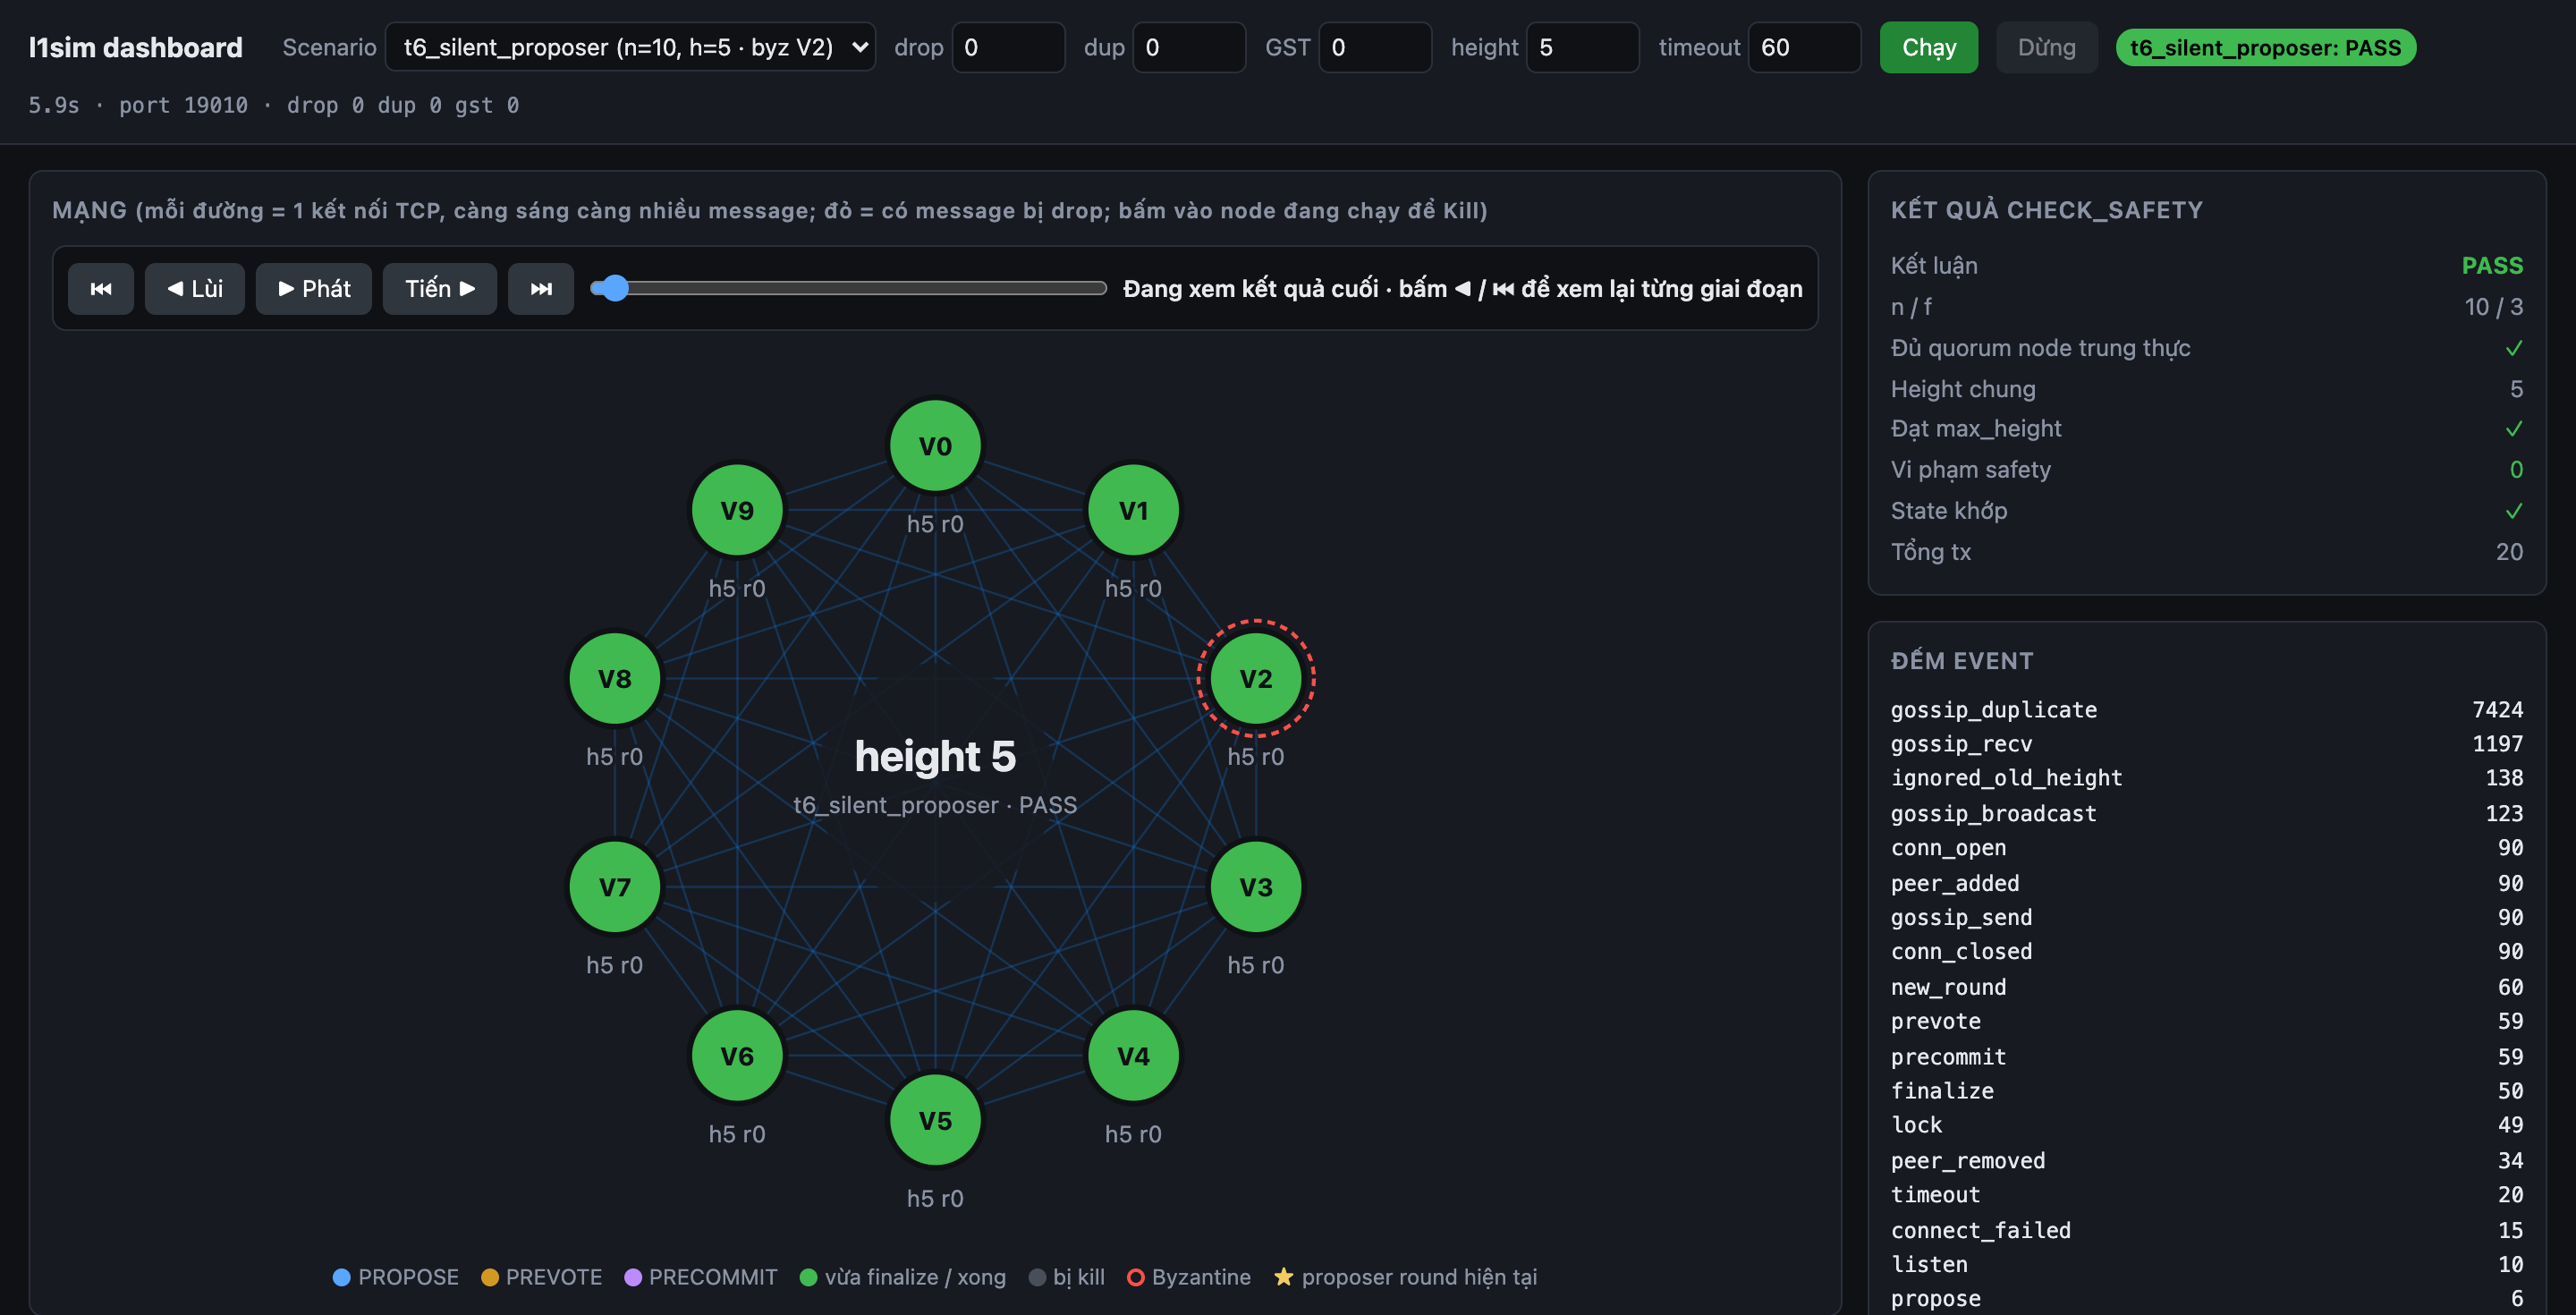
\includegraphics[width=\linewidth]{demo-ketqua.png}
\caption{Dashboard sau khi chạy T6: mạng 10 node và kết quả \code{check\_safety} (PASS).}
\label{fig:demo-kq}
\end{figure}

Sau khi chạy xong, thanh điều khiển (về đầu, \textbf{Lùi}, \textbf{Phát}, \textbf{Tiến}, về cuối cùng thanh kéo) cho phép xem lại từng giai đoạn PROPOSE $\to$ PREVOTE $\to$ PRECOMMIT $\to$ FINALIZE của mỗi height và round (T6 có 24 giai đoạn). Hình~\ref{fig:demo-replay} là giai đoạn height 2, round 0, PREVOTE: V2 là proposer (dấu sao vàng) nhưng không gửi đề xuất, nên 9 node trung thực prevote \emph{nil}; chỉ V2 prevote cho block của chính nó. Không block nào đạt 7/10 phiếu, các node chờ timeout rồi sang round 1, nơi V3 đề xuất và block được finalize. Nhóm dùng chế độ này khi demo để giải thích trực tiếp luật vote và cơ chế timeout trên log thật.

\begin{figure}[H]
\centering
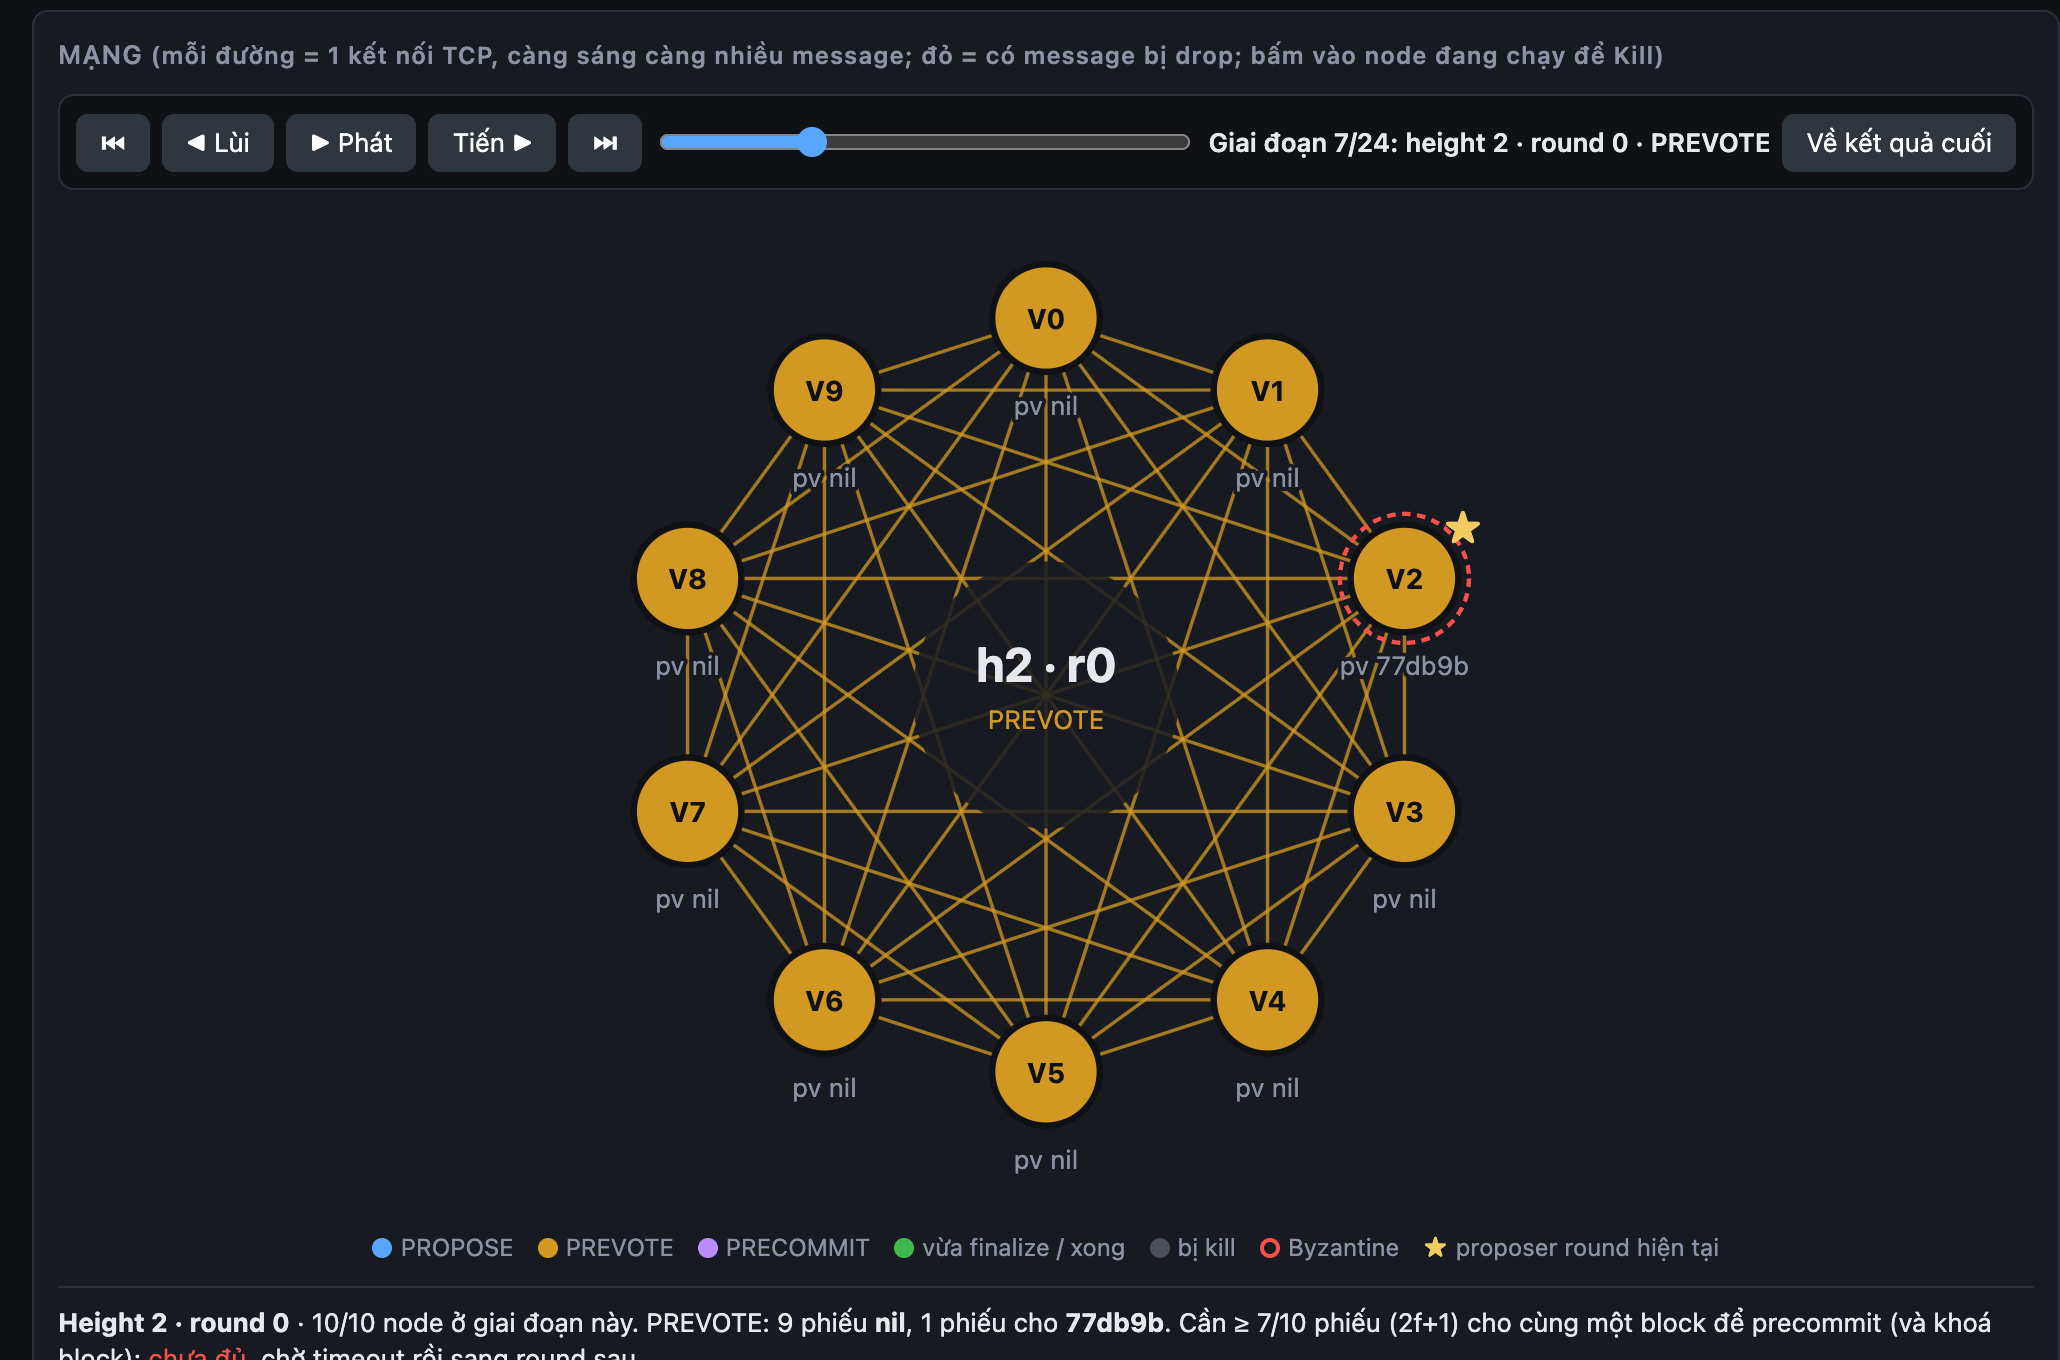
\includegraphics[width=0.6\linewidth]{demo-replay.png}
\caption{Xem lại giai đoạn height 2 · round 0 · PREVOTE của T6: 9 phiếu nil, 1 phiếu cho \code{77db9b}, chưa đủ $2f+1$.}
\label{fig:demo-replay}
\end{figure}

\subsection{T1 với giao dịch nạp sẵn và giao dịch do người dùng gửi}
Khi chạy T1 bình thường, các node \emph{không} gửi giao dịch cho nhau. Trước khi bắt đầu đồng thuận, mỗi validator tự ký 20 giao dịch của scenario và nạp vào mempool của chính nó với \code{broadcast=False}. Vì cả 10 node đều có sẵn cùng tập này, gossip thêm chỉ tạo lưu lượng trùng. Để thử đường đi thật của một giao dịch, dashboard có chế độ \textbf{chạy liên tục}: mạng vẫn nạp sẵn 20 giao dịch scenario, chạy tới khi người dùng bấm dừng, và cho phép gửi giao dịch mới (ví dụ của Alice) qua \code{l1sim.client} tới một node bất kỳ. Ở chế độ này proposer giữ đề xuất round 0 khoảng 0,6\,s, ít hơn \code{timeout\_propose} = 1\,s, để giao dịch kịp vào mempool. Bảng~\ref{tab:t1-tx} so sánh hai cách.

{\footnotesize
\renewcommand{\arraystretch}{1.1}
\begin{longtable}{@{}L{2.6cm} L{5.6cm} L{7.1cm}@{}}
\caption{Giao dịch nạp sẵn và giao dịch do người dùng gửi trong T1.}\label{tab:t1-tx}\\
\toprule
& \textbf{Nạp sẵn (T1 mặc định)} & \textbf{Người dùng gửi (Alice qua client)} \\
\midrule
\endhead
Đường đi & Gọi hàm trong process, không qua mạng & TCP tới cổng của một node: kiểm HELLO có chữ ký, gửi frame \code{TX}, chờ phản hồi \\
\rowcolor{rowgray}
Mempool & 10 node có cùng mempool ngay từ height 1 & Ban đầu chỉ node nhận có giao dịch; node đó gossip sang các node khác, và mỗi node kiểm tra lại trước khi nhận \\
Kiểm tra & \code{validate\_pending\_tx}: chữ ký $\to$ quyền sở hữu $\to$ nonce & Cùng hàm đó, chạy ở node nhận và ở từng node nhận qua gossip \\
\rowcolor{rowgray}
Phản hồi & Không có & Client nhận \code{tx\_id}, \code{accepted}, \code{reason}. \code{accepted} chỉ nghĩa là đã vào mempool, chưa phải đã commit \\
Event log & Không có event nhận giao dịch & \code{client\_tx} ở node nhận, gossip loại TX; \code{tx\_rejected} nếu bị từ chối \\
\rowcolor{rowgray}
Height của giao dịch & Cố định: 20 giao dịch nằm ở height 1--5, mỗi block 4 giao dịch & Phụ thuộc thời điểm gửi: giao dịch chỉ vào block khi proposer của round đó đã có nó trong mempool \\
Tái lập (T8) & Cùng seed thì cùng block hash và state hash & Không đảm bảo, vì height và block hash phụ thuộc lúc người dùng gửi \\
\bottomrule
\end{longtable}}

Điều kiện PASS của T1 không đổi: mọi node trung thực finalize cùng block ở mọi height và có cùng state hash. Khi nhóm thử chế độ chạy liên tục, giao dịch hợp lệ của Alice được commit ở height sau cùng lúc trên cả 10 node. Bản sửa chữ ký bị từ chối với \code{bad\_signature}, bản ký bằng domain \code{HEADER} bị từ chối với \code{wrong\_domain}, và bản gửi lại giao dịch đã commit bị từ chối vì sai nonce. Giao dịch của người lạ (Mallory, không có trong genesis) bị từ chối với \code{bad\_signature}. Kill một node trong lúc chạy thì giao dịch vẫn được commit, và \code{check\_safety} khi dừng mạng vẫn cho PASS. Khác biệt duy nhất trong verdict là \code{total\_txs} bằng 20 cộng số giao dịch của người dùng đã commit. Như vậy nạp sẵn dùng để chấm T1 và T8 vì kết quả tái lập được, còn đường client dùng để kiểm phần nhận giao dịch và các guard của nó, vốn không xuất hiện khi mọi giao dịch đều hợp lệ và có sẵn.

% ============================== TÀI LIỆU ==============================
\begin{thebibliography}{9}\small
\setlength{\itemsep}{0pt}
\bibitem{lab} Đề bài \emph{Lab01 -- Minimal Layer-1 Blockchain}, môn Blockchain, Trường ĐH Khoa học Tự nhiên, ĐHQG-HCM, 2026.
\bibitem{tm} E. Buchman, J. Kwon, Z. Milosevic. \emph{The latest gossip on BFT consensus}. arXiv:1807.04938, 2018. \url{https://arxiv.org/abs/1807.04938}
\bibitem{tmspec} CometBFT (Tendermint) Consensus Specification. \url{https://docs.cometbft.com/v0.38/spec/consensus/}
\bibitem{dls} C. Dwork, N. Lynch, L. Stockmeyer. \emph{Consensus in the presence of partial synchrony}. Journal of the ACM 35(2), 1988.
\bibitem{pbft} M. Castro, B. Liskov. \emph{Practical Byzantine Fault Tolerance}. OSDI 1999.
\bibitem{ed} S. Josefsson, I. Liusvaara. \emph{RFC 8032: Edwards-Curve Digital Signature Algorithm (EdDSA)}. IETF, 2017. \url{https://www.rfc-editor.org/rfc/rfc8032}
\bibitem{book} A. Narayanan, J. Bonneau, E. Felten, A. Miller, S. Goldfeder. \emph{Bitcoin and Cryptocurrency Technologies}. Princeton University Press, 2016.
\bibitem{crypto} Python \code{cryptography} -- Ed25519. \url{https://cryptography.io/en/latest/hazmat/primitives/asymmetric/ed25519/}
\bibitem{asyncio} Python \code{asyncio} -- Streams. \url{https://docs.python.org/3/library/asyncio-stream.html}
\end{thebibliography}

\end{document}
